% SIAM Article Template
\documentclass[onefignum,onetabnum]{siamart171218}

% Information that is shared between the article and the supplement
% (title and author information, macros, packages, etc.) goes into
% ex_shared.tex. If there is no supplement, this file can be included
% directly.

% SIAM Shared Information Template
% This is information that is shared between the main document and any
% supplement. If no supplement is required, then this information can
% be included directly in the main document.


% Packages and macros go here
\usepackage{lipsum}
\usepackage{amsfonts}
\usepackage{graphicx}
\usepackage{epstopdf}
\usepackage{algorithmic}
\ifpdf
  \DeclareGraphicsExtensions{.eps,.pdf,.png,.jpg}
\else
  \DeclareGraphicsExtensions{.eps}
\fi

%INTERNAL
\usepackage{cite}
\usepackage{amsmath,amssymb,amsfonts}
\usepackage{algorithmic}
\usepackage{graphicx}
\usepackage{textcomp}
\usepackage{siunitx}
\usepackage{url}
\usepackage{booktabs}
\usepackage{colortbl}
\usepackage{xcolor}
%\colorlet{tablerowcolor}{yellow!10} % Table row separator colour = 10% gray
\newcommand{\rowcol}{\rowcolor{tablerowcolor}} %
\let\vec\mathbf %Nicer vectors typesetting
\usepackage{color} %For authors notes to be resolved
\newcommand{\RED}[1]{\textcolor{red}{#1}}
\newcommand{\BLUE}[1]{\textcolor{blue}{#1}}
\newcommand{\GREEN}[1]{\textcolor{green}{#1}}
\newcommand{\figref}[1]{Figure~\ref{#1}}
\newcommand{\INTEGRAL}[3]{\int\limits#1 \! #2 \, \mathrm{d} #3}
\DeclareMathOperator{\atantwo}{atan2}





% Add a serial/Oxford comma by default.
\newcommand{\creflastconjunction}{, and~}

% Used for creating new theorem and remark environments
\newsiamremark{remark}{Remark}
\newsiamremark{hypothesis}{Hypothesis}
\crefname{hypothesis}{Hypothesis}{Hypotheses}
\newsiamthm{claim}{Claim}

% Sets running headers as well as PDF title and authors
\headers{Cutting Voxel Projector}{V. Kulvait, J. Moosmann and G. Rose}

% Title. If the supplement option is on, then "Supplementary Material"
% is automatically inserted before the title.
\title{Cutting Voxel Projector a New Approach to Construct 3D Cone Beam CT Operator\thanks{
Preprint pre submission as of 25 November 2024
%to SIAM Journal on Imaging Sciences on
\funding{This work was partially funded by the German Federal Ministry of Education and Research through the Research Campus STIMULATE (grant number 13GW0473A) and supported by the Hereon project \textit{Holistic Data Analysis (HoliDAy)} under the I\textsuperscript{2}B Innovation, Information \& Biologisation Fund.}
}}

% Authors: full names plus addresses.
\author{Vojt\v{e}ch~Kulvait\thanks{Institute of Materials Physics, Helmholtz-Zentrum Hereon, Max-Planck-Straße 1, 21502 Geesthacht, Germany (\email{vojtech.kulvait@hereon.de},+49 4152 871054).}
\and Julian~Moosmann\thanks{Institute of Materials Physics, Helmholtz-Zentrum Hereon, Max-Planck-Straße 1, 21502 Geesthacht, Germany (\email{julian.moosmannt@hereon.de},+49 4152 871048).}
\and Georg~Rose\thanks{Institute for Medical Engineering and Research Campus STIMULATE, Otto von Guericke University Magdeburg, Universitätsplatz 2,39106 Magdeburg (\email{georg.rose@ovgu.de},+49 3916 758862).}}

\usepackage{amsopn}
\DeclareMathOperator{\diag}{diag}


%% Added on Overleaf: enabling xr
\makeatletter
\newcommand*{\addFileDependency}[1]{% argument=file name and extension
  \typeout{(#1)}% latexmk will find this if $recorder=0 (however, in that case, it will ignore #1 if it is a .aux or .pdf file etc and it exists! if it doesn't exist, it will appear in the list of dependents regardless)
  \@addtofilelist{#1}% if you want it to appear in \listfiles, not really necessary and latexmk doesn't use this
  \IfFileExists{#1}{}{\typeout{No file #1.}}% latexmk will find this message if #1 doesn't exist (yet)
}
\makeatother

\newcommand*{\myexternaldocument}[1]{%
    \externaldocument{#1}%
    \addFileDependency{#1.tex}%
    \addFileDependency{#1.aux}%
}
%%% END HELPER CODE
%%% Local Variables: 
%%% mode:latex
%%% TeX-master: "ex_article"
%%% End: 


% Optional PDF information
\ifpdf
\hypersetup{
  pdftitle={Cutting Voxel Projector},
  pdfauthor={V. Kulvait, J. Moosmann and G. Rose}
}
\fi

% The next statement enables references to information in the
% supplement. See the xr-hyperref package for details.

%% Use \myexternaldocument on Overleaf
%\myexternaldocument{ex_supplement}

% FundRef data to be entered by SIAM
%<funding-group>
%<award-group>
%<funding-source>
%<named-content content-type="funder-name"> 
%</named-content> 
%<named-content content-type="funder-identifier"> 
%</named-content>
%</funding-source>
%<award-id> </award-id>
%</award-group>
%</funding-group>

\begin{document}

\maketitle

\begin{abstract}
In this paper, we introduce a novel class of projectors for 3D cone beam tomographic reconstruction. Analytical formulas are derived to compute the relationship between the volume of a voxel projected onto a detector pixel and its contribution to the line integral of attenuation recorded by that pixel. Based on these formulas, we construct a near-exact projector and backprojector, particularly suited for algebraic reconstruction techniques and hierarchical reconstruction approaches with nonuniform voxel grids. Unlike traditional projectors, which assume a uniform grid with fixed voxel sizes, our method enables local refinement of voxels, allowing for adaptive grid resolution and improved reconstruction quality in regions of interest. We have implemented this cutting voxel projector along with a relaxed, speed-optimized version and compared them to two established projectors: a ray-tracing projector based on Siddon's algorithm and a TT footprint projector. Our results demonstrate that the cutting voxel projector achieves higher accuracy than the TT projector, especially for large cone beam angles. Furthermore, the relaxed version of the cutting voxel projector offers a significant speed advantage over current footprint projector implementations, while maintaining comparable accuracy. In contrast, Siddon's algorithm, when achieving similar accuracy, is considerably slower than the cutting voxel projector. All algorithms are implemented in an open-source framework for algebraic reconstruction using OpenCL and C++, optimized for efficient GPU computation.
\end{abstract}

% REQUIRED
\begin{keywords}
  Cone beam computed tomography, CT reconstruction, CT projection, CT operator, Algebraic CT reconstruction, Cutting voxel projector, GPU optimized reconstruction, OpenCL, GPU computing, parallel processing
\end{keywords}

% REQUIRED
\begin{AMS}
  65D18, 65R32, 65Y05, 68U10, 44A12
\end{AMS}

\section{Introduction}

Tomographic reconstruction is a problem of inverting Radon transformation in 2D or 3D in order to recover unknown attenuation $\mu(.)$ from the set of line integrals that represents measured data. Analytical methods are based on a direct expression for the inverse or an approximation of it, see \cite{Feldkamp1984, Tuy1983, Katsevich2004}. Analytical formulas do not include discretization, which must be considered separately.

Algebraic methods, on the other hand, rely on the formulation of a projection operator that models X-ray absorption and accounts for discretization. The CT operator $\mathbf{A} \in \mathbb{R}^{m \times n}$ directly describes the relationship between the voxel attenuation values in the imaged sample $\vec{x} \in \mathbb{R}^n$ and the pixel values on the detector $\vec{b} \in \mathbb{R}^m$ so that
\begin{equation}
    \mathbf{A} \vec{x} = \vec{b}.
    \label{eq:fundament}
\end{equation}
Algebraic methods aim to compute the vector $\vec{x}_{min}$ that minimizes certain functional, such as the squared residual error for given projection data $\boldsymbol{b}$, using an iterative process, see \cite{Rit2014,Kulvait2021}. The possibility to choose the proper search space for the solution, together with the variability of the form of the functional to minimize makes these methods a versatile tool for CT reconstruction. They are suitable for applications such as limited-angle reconstruction, a priori knowledge problems or time-dependent reconstruction of contrast agent dynamics in perfusion imaging, see for example \cite{Kulvait2022,Haseljic2021}.
%in various circumstances such as limited angle reconstruction, problems with apriori knowledge or the reconstruction of the time dependent contrast agent dynamics in scope of perfusion imaging, see for example \cite{Haseljic2021}.%, see for example \cite{}.

\begin{figure}
    \centering
    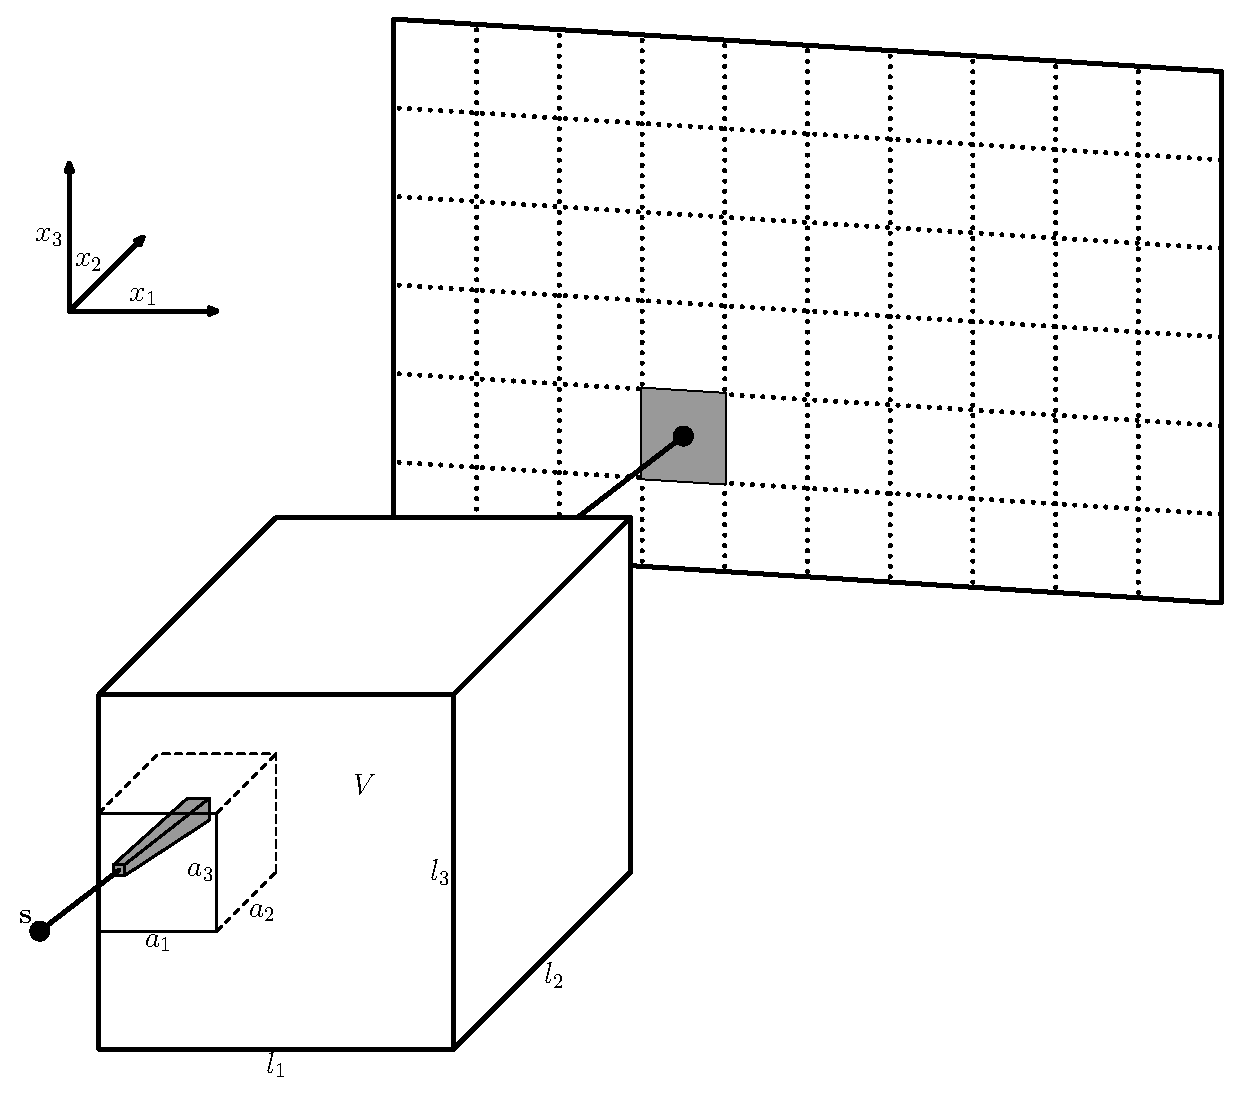
\includegraphics[width=0.45\textwidth]{projectionScheme-1.eps}
    \caption{The cutting voxel projector estimates the voxel contribution to the detected value at a particular pixel based on the volume of intersection of the voxel with all possible rays to that pixel.}
    \label{fig:problem_setup}
\end{figure}

Iterative methods require efficient and accurate evaluation of the actions of projection and backprojection operators. The projection operator acts on volume data $\vec{x}_{\mathrm{IN}} \in \mathbb{R}^n$  and returns the projection vector $\vec{b}_{\mathrm{OUT}} \in \mathbb{R}^m$ such that $\vec{b}_{\mathrm{OUT}} = \mathbf{A} \vec{x}_{\mathrm{IN}}$. The backprojection operator acts on projection vector $\vec{b}_{\mathrm{IN}} \in \mathbb{R}^n$ and returns the volume data $\vec{x}_{\mathrm{OUT}} \in \mathbb{R}^n$ such that $\vec{x}_{\mathrm{OUT}} = \mathbf{A}^\top \vec{b}_{\mathrm{IN}}$. Because the I/O latencies of data storage devices are high, it is prohibitive for typical CT systems to store the matrix $\mathbf{A}$ on disk and perform these matrix multiplications directly. Computing the projection and backprojection operators on the fly on current GPUs is typically orders of magnitude faster than working with the $\mathbf{A}$ matrix stored on disk. Therefore, there is a demand for fast and accurate projection and backprojection operators.

Ray casting/tracing projectors are well established not only in the context of CT imaging, but also in the context of computer graphics, see \cite{Siddon1985,Sramek2000,Zhao2003}. They track the ray cast from the source to the detector and add the values along the way to form the product of the geometry factors in $\mathbf{A}$ row with given vector of attenuation $\vec{x}_{\mathrm{IN}}$. Outer loop of these projectors is over the detector pixels, so they are scanning the matrix $\mathbf{A}$ row by row. Their accuracy is strongly dependent on the number of rays cast. Backprojection is typically slower than projection and, in addition, it is unable to capture the underlying physical process well, resulting in a strong geometric artefacts in reconstructions.

Footprint projectors on the other hand try to estimate for each voxel and position on the detector the length of the intersection of the voxel with the ray to that position. Their outermost loop is over voxels, so that they scan the matrix $\mathbf{A}$ column by column. Current implementations rely on the assumption that footprints can be approximated in each detector direction by very simple functions, for example by constants with a small support, see \cite{Man2004}, or by constants in the middle with linearly decaying tails on each side, so-called trapezoidal functions. Separable footprint projectors approximate blur on the detector due to a given voxel by product of two such functions, each for one detector dimension, see \cite{Long2010}. They extend the work of \cite{Man2004} and are considered state of the art CT projectors. The inaccuracies of this class of projectors are due to the fact that the actual footprints are generally not separable and thus do not satisfy assumptions about the shape of the footprint functions.
% The algorithm \cite{Long2010} also assumes certain geometric setting of the acquisition system. 

In this paper, we construct a projector that directly describes the voxel pixel correspondence by computing integrals over the volumes of voxel cuts projected onto a given pixel instead of averaging line integrals over rays passing through the voxels, see \figref{fig:problem_setup}. In order to accurately compute the projection of a given voxel onto a given pixel, we need to reformulate the problem using integral calculus to find the correspondence between the integrals over all rays passing through the voxel and the integrals over the voxel cut volume. This approach eliminates the need to cast a high number of rays towards a given pixel to increase accuracy, and also overcomes assumptions about the shapes of the footprints.

\section{Problem formulation}
\label{sec:formulation}
In this section we derive fast, almost exact projector for 3D cone beam geometry. We use linear Lambert-Beer law to compute pixel signal based on the known function $\mu : \mathbb{R}^3 \to \mathbb{R}^+_0 $ that represents the attenuation. We emphasize that instead of direct integration of the attenuation over the rays to the detector we find a mathematical transformation to integrate attenuation over the subvolumes of voxels projected to given pixel.

\subsection{Geometry discretization}
Throughout the paper, we will use the following standard assumptions about the discretized problem. Let's the X-ray source, object to be scanned and the detector be located in the Euclidean space $\mathbb{R}^3$. The X-ray source at given time $t$ has coordinates  $\vec{s} = (s_1, s_2, s_3)$. The object to be scanned lies inside a rectangular box $V$ centered at $(0,0,0)$ with the edge lengths $(l_1, l_2, l_3) \in \mathbb{R}_{+}^3$. Box $V$ represents the volume to be projected
\begin{equation}
    V = \{ \vec{x} \in \mathbb{R}^3 : |x_1| < \frac{l_1}{2},|x_2| < \frac{l_2}{2}, |x_3| < \frac{l_3}{2} \}.
    \nonumber
\end{equation}
The discretization is given by the voxel sizes $(a_1,a_2,a_3) \in \mathbb{R}_{+}^3$ and number of the voxels per edge $(N_1, N_2, N_3) \in \mathbb{N}^3$. For the dimension compatibility it is required that $a_\alpha N_\alpha = l_\alpha$ for $\alpha \in \{1,2,3\}$. Let's denote the center of the voxel $(0,0,0)$ by 
\begin{equation}
    \vec{x}^{(0,0,0)} =  (\frac{-l_1 + a_1}{2}, \frac{-l_2 + a_2}{2}, \frac{-l_3+a_3}{2}).
    \nonumber
\end{equation}
The center of the general voxel $(i,j,k)$,  $i\in \{0...N_1-1\}$, $j\in \{0...N_2-1\}$ and $k\in \{0...N_3-1\}$ is then
\begin{equation}
    \vec{x}^{(i,j,k)} = \vec{x}^{(0,0,0)} +  (i a_1, j a_2, k a_3),
    \nonumber
\end{equation}
and the volume of the voxel is given by
\begin{equation}
V^{(i,j,k)} = \{ \vec{x} \in \mathbb{R}^3 : |x_\alpha-x^{(i,j,k)}_\alpha| < \frac{a_\alpha}{2}, \alpha \in \{1,2,3\} \}.
\nonumber
\end{equation}
The attenuation $\mu : \mathbb{R}^3 \to \mathbb{R}^+_0 $  has a support on $V$ and is constant on each voxel so that
\begin{equation}
\forall \vec{x} \in V^{(i,j,k)} \quad \mu(\vec{x}) = \mu^{i,j,k}.
\nonumber
\end{equation}

\subsection{Detector discretization}
In what follows, we consider flat panel detector with the rectangle shaped pixels without gaps. Detector surface is parametrized by means of two Euclidean coordinates $\chi = (\chi_1, \chi_2) \in \mathbb{R}^2$. These assumptions allow us to clearly explain main concepts, yet it is straightforward to relax them and consider curved detectors, differently shaped pixels and gaps between pixels. In the current implementation, to compute the cuts, we additionally assume that the $x_3$ axis of the global geometry is parallel to the $\chi_2$ axis of the detector, see Figure \ref{fig:carmconventionalsetup}. However, this assumption is not essential to derive the main formula for the cutting voxel projector in this chapter.

Let's assume that $(M, N) \in \mathbb{N}^2$ are the counts of the pixels per edge and the spacing of pixels is given by $(b_1,b_2) \in \mathbb{R}_{+}^2$. The center of the pixel $(0,0)$ is $\vec{\chi}^{(0,0)} =  (0, 0)$. The center of the general pixel $(m,n)$,  $m\in \{0...M-1\}$ and $n\in \{0...N-1\}$ is at
\begin{equation}
    \vec{\chi}^{(m,n)} = \vec{\chi}^{(0,0)} +  (m b_1, n b_2)
\end{equation}
and the surface of the pixel is parametrized as
\begin{equation}
A^{(m,n)} = \{ \vec{\chi} : |\chi_\alpha-\chi^{(m,n)}_\alpha| < \frac{b_\alpha}{2}, \alpha \in \{1,2\} \}.
\end{equation}

\subsection{Parametrization of the rays and attenuation model}

To define the geometry of the system, we begin by fixing the positions of the source and detector. Using these fixed points, we introduce a spherical coordinate system denoted by $(r, \theta, \varphi) \in [0,\infty] \times [0,\pi/2] \times [0,2\pi)$, which which originates at the source position and provides a natural way to describe the rays from the source to the particular detector position. The zenith denotes the direction with zero inclination $\theta = 0$, which corresponds to the principal ray that is the ray orthogonal to the flat panel detector. The intersection of the detector with the principal ray is called the principal point $\vec{\chi}^{P} =  (\chi_1^P, \chi_2^P)$. Rays with azimuth $\varphi = 0$ are projected onto a semi-line on the detector starting at a principal point parallel to the $\chi_1$ axis.

For a given view, there is an exact correspondence between this local spherical coordinate system and the global coordinate system. We can introduce an auxiliary Euclidean system $(\tilde{x}_1, \tilde{x}_2, \tilde{x}_3)$ centered at $\vec{s}$ and the transformation given by orthogonal $3 \times 3$ matrix $Q$ such that 
\begin{equation}
    \tilde{\vec{x}} = Q (\vec{x} - \vec{s}).
\end{equation}
The rotation $Q$ transforms the axes so that $x_1$ is parallel to the detector coordinate $\chi_1$, $x_2$ is parallel to $\chi_2$ and $x_3$ is in the direction of the normal from the source to the detector, see Figure \ref{fig:flat_panel}.
The system $(\tilde{x}_1, \tilde{x}_2, \tilde{x}_3)$ then in turn induces local spherical coordinate system in a way that
\begin{align}
    r &= \sqrt{\tilde{x}_1^2 + \tilde{x}_2^2 + \tilde{x}_3^2},\\
    \theta &= \arccos \frac{\tilde{x}_3}{\sqrt{\tilde{x}_1^2 + \tilde{x}_2^2 + \tilde{x}_3^2}},\\
    \varphi &= \atantwo (\tilde{x}_2, \tilde{x}_1).
\end{align}

\begin{figure}
    \centering
    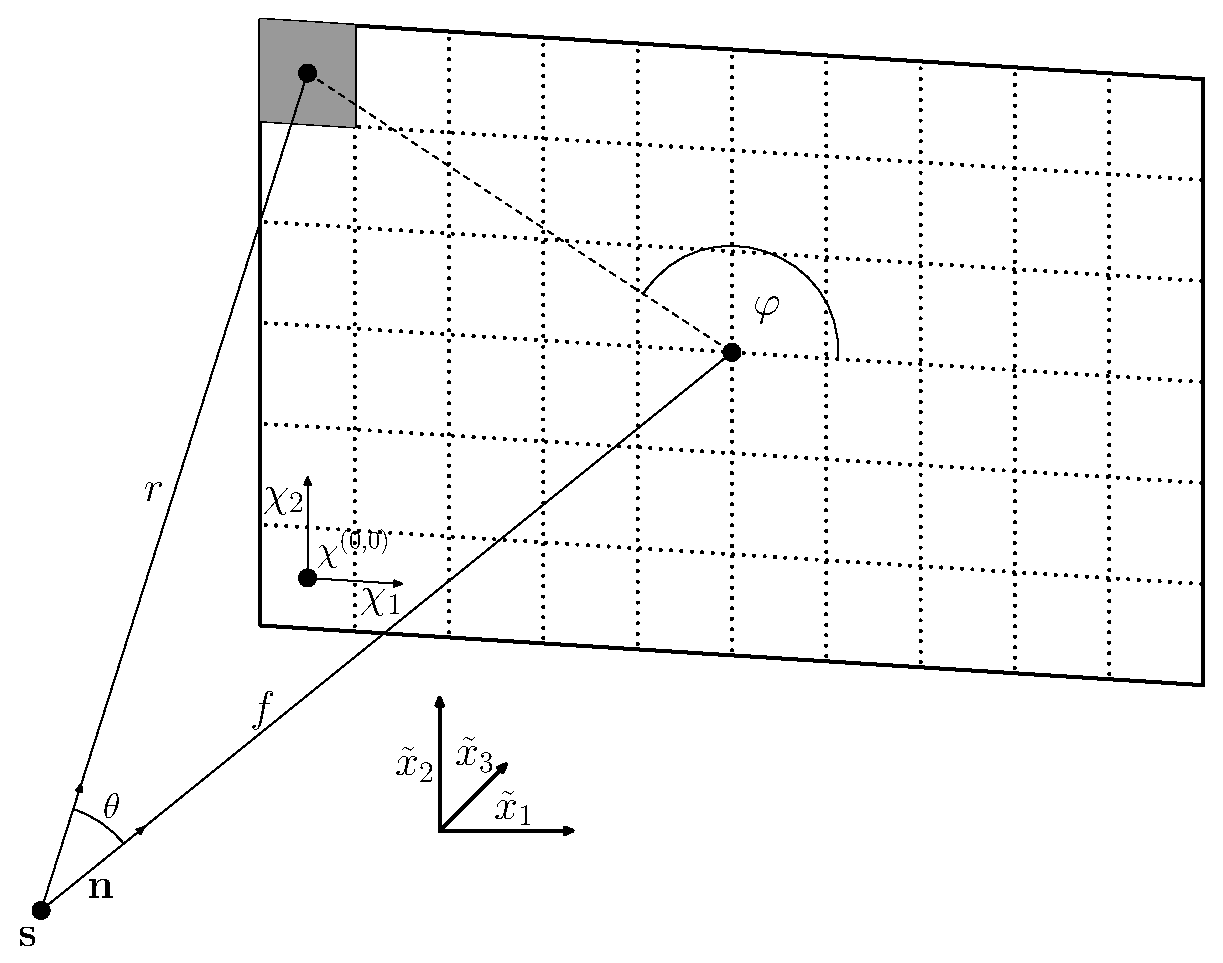
\includegraphics[width=0.45\textwidth]{auxiliaryLocalCoordinatesV05.eps}
    \caption{Auxiliary local Euclidean coordinates for a given view that induce a local spherical coordinate system. Coordinate $\theta$ is the cone angle.}
    \label{fig:flat_panel}
\end{figure}

The model given by Lambert-Beer law and the cone beam geometry maps the lines in $\mathbb{R}^3$ starting at the source position $\vec{s}$ to the integrals over the attenuation $\mu$ along these lines. The lines can be parametrized by polar and azimuthal angles in spherical coordinate system $[\theta, \varphi] \in [-\pi/2,\pi/2] \times [0,2\pi)$. Let's $\vec{L}[\theta, \varphi]: \mathbb{R} \to \mathbb{R}^3$ define a isometric parametrization $\vec{L}[\theta, \varphi](q), q \in [0, \infty)$ of the ray  in the direction $[\theta, \varphi]$ such that $\vec{L}[\theta, \varphi](0) = \vec{s}$. 

We identify the coordinates $\chi = (\chi_1, \chi_2) \in \mathbb{R}^2$ with the parameters $\theta,\varphi$, which define the line line through the source $L[\theta,\varphi](.)$ that hits the detector at $(\chi_1, \chi_2)$. 
We consider $[\theta,\varphi]$ or $[\chi_1, \chi_2]$ just two different parametrizations of the  set of all lines passing through the $\vec{s}$. In the projective geometry such set is called projective plane or projective space of dimension two, see \cite{Prasolov2001}.

Consider the ray in the direction $[\theta, \varphi]$. According to Lambert-Beer law the X-ray intensity after passing the scanned object measured on the detector is
\begin{equation}
    I(\theta, \varphi) = I_0(\theta, \varphi) \exp{\left(-\INTEGRAL{_0^\infty}{\mu(\vec{L}[\theta, \varphi]( q))}{q}\right)}, \label{eq:lambertbeer}
\end{equation}
where $I_0(\theta, \varphi)$ is the blank scan intensity that would be measured at the same detector position without scanned object. The quantity
\begin{equation}
    E(\theta, \varphi) \stackrel{1}{=} \ln(I_0(\theta, \varphi)) - \ln(I(\theta, \varphi)) \stackrel{2}{=} \INTEGRAL{_0^\infty}{ \mu(\vec{L}(\theta, \varphi, q))}{q}
    \label{eq1:extinciton}
\end{equation}
is in what follows called \textbf{extinction}. It is not common terminology and sometimes it is refereed just as negative logarithm of transmission or line integral of attenuation. When referring to the discretized tomographic problem \eqref{eq:fundament}, we call discretized extinction often right hand side, projection vector or vector $\vec{b}$.

\subsection{Per pixel extinction}
\label{sec:perpixel}
When scanning the volume $V$, the CT scanner measures the intensities $I^{(m,n)}$ for each view and each pixel on the detector and and then calculates the extinction values $E^{(m,n)}$ based on the known per pixel intensities $I_0^{(m,n)}$ and the first relation in \eqref{eq1:extinciton}. The values of $E^{(m,n)}$ represent the input vector $\vec{b}$ of the reconstruction problem \eqref{eq:fundament}. In order to obtain specific values within the matrix $\mathbf{A}$, the so-called geometric factors, we need to determine the specific form of the second equation in \eqref{eq1:extinciton} for the discretized extinction $E^{(m,n)}$.

A first order approximation of the relationship between voxel and pixel values is to cast rays towards the pixels and construct the CT operator as follows
\begin{equation}
    E^{(m,n)} = \sum_{i,j,k} \mu^{i,j,k} |V^{(i,j,k)} \cap \vec{L}(\chi^{(m,n)}, .))|,
    \label{eq1:discreteextinction}
\end{equation}
where $|V^{(i,j,k)} \cap \vec{L}(\chi^{(m,n)}, .))|$ is the length of the path of given ray through the given voxel. For computing these intersections, we utilize Siddon algorithm, see \cite{Siddon1985}. The problem with this approach is that the extinction value $E^{(m,n)}$ depends on the exact location on the pixel surface where the beam is cast. The solution is, for example, to create a grid of $K \times K$ equally spaced points on the pixel surface and average all extinction values in \eqref{eq1:discreteextinction} with respect to the rays thrown towards the grid points. We will henceforth refer to the algorithm obtained in this way as \texttt{SiddonK}, i.e., for example, \texttt{Siddon8} casts 64 rays towards each pixel.

To robustly estimate the extinction over pixels, we use the following formula using the integral over the pixel area, which can also be obtained as a limit process derived from the sum over grid points in the \texttt{SiddonK} algorithm if we send $K$ to infinity.
\begin{equation}
    E^{(m,n)} = \frac{e^{(m,n)}}{a^{(m,n)}},\label{eq1:integ}
\end{equation}
where
\begin{equation}
    e^{(m,n)} = \int_{\chi \in A^{(m,n)}} \sum_{i,j,k} \mu^{i,j,k} \mathcal{D}(\chi, i, j, k)  \,dS(\chi), \label{eq1:voxat}
\end{equation}
is the total extinction over the area of the pixel,
\begin{equation}
\mathcal{D}(\chi, i, j, k)  = |V^{(i,j,k)} \cap \vec{L}(\chi, .))|
\end{equation}
is the length of the path of the ray parametrized by $\chi$ through voxel $(i,j,k)$ and
\begin{equation}
    a^{(m,n)} = \int_{\chi \in A^{(m,n)}} 1  \,dS(\chi).
    \label{eq:area}
\end{equation}
The integrals \eqref{eq1:voxat} and \eqref{eq:area} are over the parameterization $\,dS(\chi)$ of the infinitesimal detector surface at point $\chi$ in world coordinates, so that $a^{(m,n)}$ is the area of a given pixel.

Alternatively, we can transform the problem to the unit ball. As we noted $(\theta, \varphi)$ can be also understood as a discretization of unit ball centered at the source position $\vec{s}$. Therefore for given pixel we can integrate \eqref{eq1:extinciton} along $(\theta, \varphi)$ that maps to a given pixel and divide by the surface of the unit ball that maps to that pixel. We have the formula
\begin{equation}
    \bar{E}^{(m,n)} = \frac{\bar{e}^{(m,n)}}{\bar{a}^{(m,n)}},\label{eq1:integub}
\end{equation}
where
\begin{equation}
    \bar{e}^{(m,n)} = \int\limits_{(\theta, \varphi) \in A^{(m,n)}}  \sum_{i,j,k} \mu^{i,j,k} \mathcal{D}(\theta, \varphi, i, j, k) \sin\theta \mathrm{d}\theta \mathrm{d}\varphi \label{eq1:voxatub}
\end{equation}
is the total extinction over the area of the unit ball segment
\begin{equation}
    \bar{a}^{(m,n)} = \int\limits_{(\theta, \varphi) \in A^{(m,n)}}  \sin\theta d\,\theta d\,\varphi.\label{eq1:voxsurfub}
\end{equation}
Here we utilize formula for the unit ball surface element being $dS = \sin\theta d\,\theta d\,\varphi$. 


\subsection{Cutting voxel projector}

To derive new strategy to compute \eqref{eq1:integ} or \eqref{eq1:integub}, we transform integrals over the area of detector cells in \eqref{eq1:voxat} and \eqref{eq1:voxatub} into the integrals over the volume of the voxels of the type
\begin{equation}
    \int_V \mu(\vec{x})\,dx. \label{eqx:volint}
\end{equation}
Using this approach, instead of averaging the ray path length over a voxel, we can then calculate the voxel volume projected onto a given pixel and derive the extinction increment from this value. We start by rewriting the integral \eqref{eq1:voxat} into the form
\begin{equation}
    e^{(m,n)} = \sum_{i,j,k} \mu^{i,j,k} e_{i,j,k}^{(m,n)},
\end{equation}
where
\begin{equation}
     e_{i,j,k}^{(m,n)} = \int_{\chi \in A^{(m,n)}}  |V^{(i,j,k)} \cap \vec{L}(\chi, .)| \,dS(\chi).\label{eq1:svi}
\end{equation}
Let's define an indicator function that tests if the line at the point given by the local spherical coordinates introduced in Figure \ref{fig:flat_panel}, intersects the voxel
\begin{equation}
\vec{I}^{i,j,k}(r, \theta, \varphi) = 
\begin{cases} 1 \quad \mbox{if } \vec{L}(\theta, \varphi, r) \in V^{(i,j,k)} \\
0 \quad \mbox{elsewhere.} \end{cases}
\label{eq:indicator}
\end{equation}
Applying \eqref{eq:indicator}, we rewrite the length of the voxel ray intersection in \eqref{eq1:svi} as
\begin{equation}
    |V^{(i,j,k)} \cap \vec{L}(\chi, .)| = \int_0^\infty \vec{I}^{i,j,k}(r, \theta(\chi), \varphi(\chi)) d\,r.
    \label{eq:rayintegral}
\end{equation}
The surface element in spherical coordinates is $\mathrm{d}\tilde{S}(\chi) = R^2 \sin{\theta} \,\mathrm{d}\theta \,\mathrm{d}\varphi$, where $R$ is the distance of a given pixel on the detector from the source. We assume that the pixel is small enough so that $R$ over its  area can be approximated by a constant value, and also that the curvature of the spherical coordinates on its surface can be ignored so that the angle between the pixel and the element $\mathrm{d}\tilde{S}(\chi)$ is constant. The element $\mathrm{d}\tilde{S}(\chi)$ is perpendicular to the ray so that the angle of its normal with the normal to the pixel is $\theta$, the cone angle. The correction for integration over the surface element of a pixel is therefore of the form $\mathrm{d}\tilde{S}(\chi) = \cos{\theta} \,\mathrm{d}S(\chi)$. Combining this equality with \eqref{eq1:svi} and \eqref{eq:rayintegral} yields
\begin{equation}
     e_{i,j,k}^{(m,n)} = \INTEGRAL{_0^\infty}{\int\limits_{\chi \in A^{(m,n)}} \vec{I}^{i,j,k}(r, \varphi(\chi), \theta(\chi)))  R^2 \frac{\sin{\theta}}{\cos{\theta}} \,d\theta \,d\varphi }{r}.\label{eq1:svx}
\end{equation}

Volume element in spherical coordinates has a form
\begin{equation}
    dV = r^2 \sin{\theta} \,d\theta \,d\varphi \,dr
\end{equation}
so the integral \eqref{eq1:svx} can be rewritten to the form 
\begin{equation}
     e_{i,j,k}^{(m,n)} = \int_{V^{(i,j,k)}_{(m,n)}} \frac{R^2}{r^2\cos{\theta}}  \,dV,
     \label{eq:extinction}
\end{equation}
where $V^{(i,j,k)}_{(m,n)}$ is a intersection of voxel $(i, j, k)$ with all rays to the pixel $(m,n)$. 
We assume that $\cos{\theta}$ and $R$ are constant on each detector pixel and approximate them by the value in its center. When $f$ is the distance from s to the detector, we have that 
\begin{equation}
    R \cos{\theta} = f,
\end{equation}
which further simplifies \eqref{eq:extinction} into the form
\begin{equation}
     e_{i,j,k}^{(m,n)} =  \frac{f^2}{\cos^3{\theta}} \int_{V^{(i,j,k)}_{(m,n)}}  \frac{1}{r^2}  \,\mathrm{d}V
\end{equation}
and establishes the formula for the discrete extinction of the cutting voxel projector
\begin{equation}
    E^{(m,n)} = \frac{f^2}{a^{(m,n)} \cos^3{\theta}} \sum_{i,j,k} \mu^{i,j,k} \int_{V^{(i,j,k)}_{(m,n)}}  \frac{1}{r^2} d\,x. \label{cvp}
\end{equation}
Interestingly, for parallel ray geometry we do not have to use any curvilinear coordinate transform and the formula \eqref{eq:rayintegral} simplifies to the form
\begin{equation}
    E^{(m,n)}_{PR} = \frac{1}{a^{(m,n)} \cos{\hat{\theta}}} \sum_{i,j,k} \mu^{i,j,k} \int_{V^{(i,j,k)}_{(m,n)}}  1 d\,x,
    \label{eq1:extinciton_parallel}
\end{equation}
where $\hat{\theta}$ is the angle between rays and normal to the detector. For standard situation $\hat{\theta} = 0$ is then $\cos{\hat{\theta}}=1$.

For the geometry of the detector transformed to the surface of the unit sphere, we start from the integral \eqref{eq1:voxatub}. The derivation is easier because we do not have to correct for the angle mismatch of the infinitesimal element of the pixel surface and the infinitesimal element of the spherical coordinates as it is zero. The formula analogous to the integral \eqref{eq1:svx} reads
\begin{equation}
     \bar{e}_{i,j,k}^{(m,n)} = \INTEGRAL{_0^\infty}{ \int\limits_{\chi \in A^{(m,n)}} \vec{I}^{i,j,k}(r, \varphi(\chi), \theta(\chi)))  \sin{\theta} \,\mathrm{d}\theta \,\mathrm{d}\varphi}{r},
\end{equation}
With the formula for the volume element in spherical coordinates $\mathrm{d}V = r^2 \sin{\theta} \,\mathrm{d}\theta \,\mathrm{d}\varphi $ it might be concluded that
\begin{equation}
     \bar{e}_{i,j,k}^{(m,n)} =  \int_{V^{(i,j,k)}_{(m,n)}}  \frac{1}{r^2}  \,\mathrm{d}V. \label{eq1:intcut}
\end{equation}
For the computation of the area of the unit ball that gets projected to the given pixel in \eqref{eq1:voxsurfub}, we can utilize spherical trigonometry, see \cite{3540309} and \cite[p. 98-99]{Todhunter1914}. For the area of the polygon on the unit sphere we have
\begin{equation}
    \bar{a}^{(m,n)} = \alpha + \beta + \gamma + \delta - 2 \pi,  
\end{equation}
where $\alpha$, $\beta$, $\gamma$ and $\delta$ are sizes of the four polygon angles on that sphere. So let's have unit vectors $\vec{t}_0^{(m,n)}$, $\vec{t}_1^{(m,n)}$, $\vec{t}_2^{(m,n)}$, $\vec{t}_3^{(m,n)}$ in the direction of the pixel corners ordered counter clock wise. After some manipulations we can conclude
\begin{equation}
    \bar{a}^{(m,n)} = 2 \pi - \sum_{i=0}^3 \arccos{ \frac{(\vec{t}_i \times \vec{t}_{i+1})\cdot(\vec{t}_{i+1} \times \vec{t}_{i+2})}{|\vec{t}_i \times \vec{t}_{i+1}||\vec{t}_{i+1} \times \vec{t}_{i+2}|}}. 
\end{equation}
The equation \eqref{eq1:integ} became
\begin{equation}
    \bar{E}^{(m,n)} = \frac{1}{\bar{a}^{(m,n)}} \sum_{i,j,k} \mu^{i,j,k} \int_{V^{(i,j,k)}_{(m,n)}}  \frac{1}{r^2} d\,x. \label{cvpus}
\end{equation}

Equations \eqref{cvp} and \eqref{cvpus} are general forms of discrete extinction for cutting voxel projector in flat panel geometry and in the geometry transformed to a unit sphere. Note that the two formulations \eqref{cvp} and \eqref{cvpus} differ only in the form of the factor in the product for a given pixel. It is therefore possible to first calculate the sum of
\begin{equation}
    S^{(m,n)} = \sum_{i,j,k} \mu^{i,j,k} \int_{V^{(i,j,k)}_{(m,n)}}  \frac{1}{r^2} d\,x, \label{cvpsu}
\end{equation}
which is the same for both formulations and then rescale these sums at the pixel level according to the chosen formulation. 

\subsection{Volume of the voxel cuts}
To be able to use formulas \eqref{cvp} or \eqref{cvpus} we have to be able to evaluate value  $\bar{e}_{i,j,k}^{(m,n)}$ by means of the integral \eqref{eq1:intcut} for each pixel and voxel pair.

Here we assume that the voxel cuts are such small that $r^2$ is approximately constant for the whole volume $V^{(i,j,k)}_{(m,n)}$. We can estimate $r=r_{i,j,k}$ being the distance of the center of the given voxel to the source $s$ or more precisely $r=r_{i,j,k,m,n}$ being the distance of the center of mass of  $V^{(i,j,k)}_{(m,n)}$ to the source. This assumption enables us to write \eqref{eq1:intcut} in the form
\begin{equation}
    \bar{e}_{i,j,k}^{(m,n)} = \sum_{i,j,k} \frac{\mu^{i,j,k}}{r_{i,j,k,m,n}^2} |V^{(i,j,k)}_{(m,n)}|. \label{vox}
\end{equation}
This concludes the theoretical derivation of the cutting voxel projector. In the next section, we present our current implementation and describe how the calculation of the volume of voxel cuts for each voxel pixel pair is handled in it. 

\section{Implementation}
\label{sec:implementation_full}
The current cutting voxel projector implementation is part of a larger framework for CBCT reconstruction available at \url{https://github.com/kulvait/kct_cbct} developped by the first author. It is a set of tools written in C++ and OpenCL optimized to run on GPU architectures with fast local memory. The software is released under the open source license GNU GPL3.

\subsection{Calculating voxel cuts}
\label{sec:cuts}
To simplify the calculation of the voxel cuts, we assume a geometric arrangement where the $\chi_2$ axis of the detector is parallel to the $x_3$ axis of world coordinates and by convention their directions are opposite, see Figure \ref{fig:carmconventionalsetup}. This arrangement is used in most current CT trajectories, including the circular trajectory, and is also assumed by footprint projectors, see \cite{Long2010}.

\begin{figure}
    \centering
    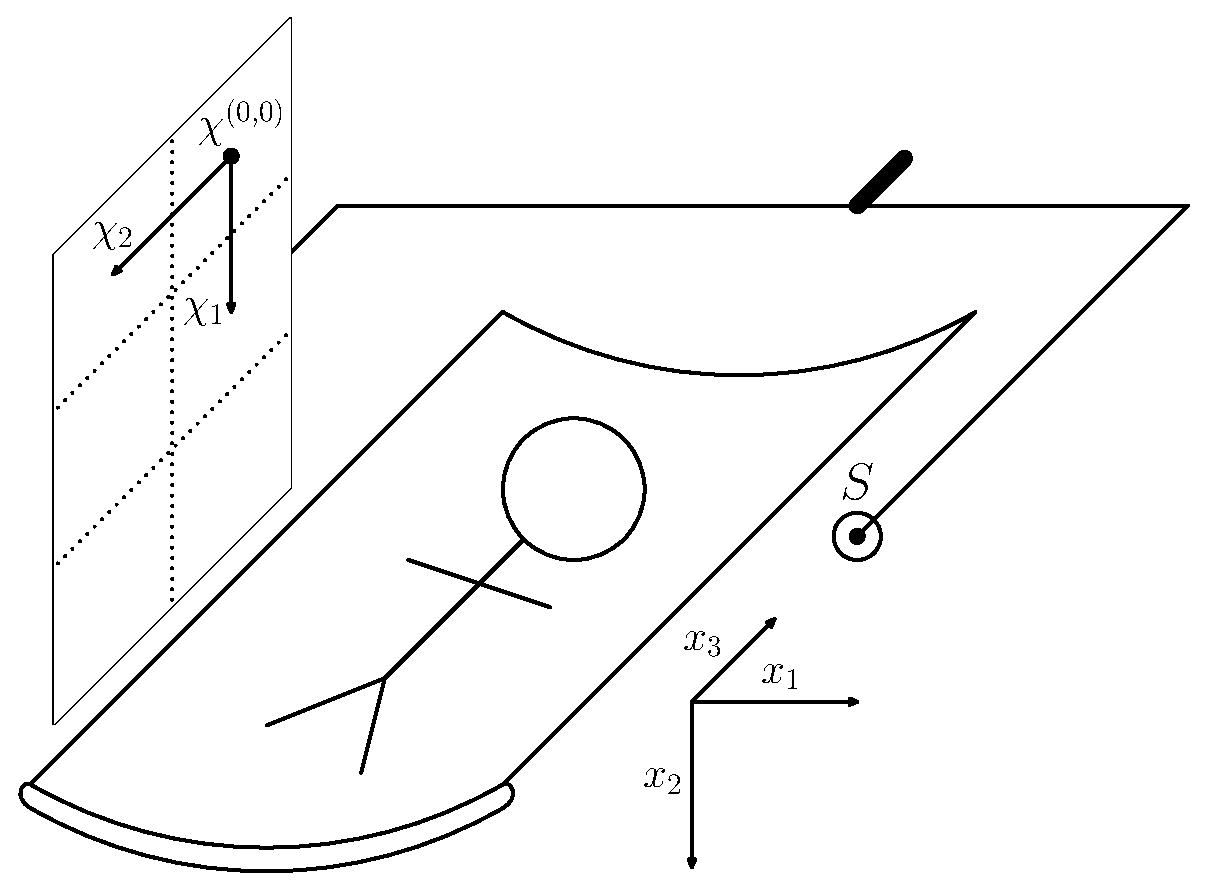
\includegraphics[width=0.45\textwidth]{CTGeometryConstraintsV05.eps}
    \caption{Geometric convention and simplification for the classical cone beam CT arrangement. The axis of rotation is parallel to the $x_3$ axis of world coordinates. In addition, the $x_3$ axis is parallel to the $\chi_2$ axis of the detector, but they have opposite orientations. The origin of the detector is placed in the center of the corner pixel. This arrangement is also assumed in the software.}
    \label{fig:carmconventionalsetup}
\end{figure}

Then, for any two points $x^I = (x_1,x_2,x_3)$ and $x^{II}= (x_1,x_2,x_3')$, which differ only in the value of the third world coordinate it holds that 
\begin{equation}
    \chi_1(x^I) = \chi_1(x^{II}). \label{eq:columnprojectionidentity}
\end{equation}
Therefore, the projection onto the $\chi_1$ is independent of the value of $x_3$. That means that the profiles of the cuts through a given voxel in the $x_1 x_2$ plane will be the same for all $x_3$ coordinates of given voxel and moreover they will be the same for all the voxels with the same fixed $i$ and $j$ indices $V^{i,j,.}$. 

Based on this observation, we first find for each voxel $V^{i,j,k}$ and coordinate $n$ on the detector the polygons $H^{i,j}_n$ into which the base of the voxel parallel with the $x_1x_2$ plane is cut by rays directed to pixels in the $n$-th column of the projector. Our current implementation first finds the corners of the voxel base with the smallest and largest projections $\chi_1^{min}$ and $\chi_1^{max}$. From this we determine the range of allowable integer values $n$ of the column indices of the pixels on the detector on which the voxel is projected. Next, for a given index $n$ we find a polygon $H-^{i, j}_n$ given by the cut of the voxel basis corresponding to projections in the range $\chi_1 \in [\chi_1^{min}, n-0.5]$ and a polygon $H+^{i, j}_n$ corresponding to projections in the range $\chi_1 \in [\chi_1^{min}, n+0.5]$. Finally, we find the polygon $H^{i, j}_n$ as the difference of the sets $H+^{i, j}_n \setminus H-^{i, j}_n$. We compute the area $A_{n}^{i,j}$ and the position of the center of the mass of these polygons being e.g. $\vec{CM}_n^{i,j} = (x_1^{CM},x_2^{CM})$. 

Then, for a given voxel, we reduce the cut in the $x_1 x_2$ plane to its center of mass and find the positions of the $x_3$ breakpoints, which correspond to the projections onto the pixel boundaries between the detector rows. Let $d^{(i,j,k)}_{(m,n)}$ estimate the $x_3$ length of the voxel cut given by the difference of two consecutive breakpoints corresponding to the $m$ row of the detector restricted to the admissible range of $x_3$ coordinates of the given voxel.  %Let's define the function $P_3: P_3(x_1, x_2, \chi_2) = \tilde{x}_3$, such that the point $(x_1, x_2, \tilde{x}_3)$ projects to the $\chi_2$ coordinate of the detector.  We then can for given center of mass compute $d^{(i,j,k)}_{(m,n)} = |[x^{(0,0,0)}_k + k a_3, x^{(0,0,0)}_k + (k+1) a_3] \cap [b(x_1^{CM},x_2^{CM}, m+1), b(x_1^{CM},x_2^{CM}, m)]|$. 
On this basis, we estimate the volume of voxels in \eqref{vox} as
\begin{equation}
    |V^{(i,j,k)}_{(m,n)}|=A_{n}^{i,j}*d^{(i,j,k)}_{(m,n)}. \label{eq:cutvolume}
\end{equation} 

To summarize, we approximate the volume of a voxel cut projected onto a given pixel as the product of its area in the $x_1 x_2$ plane and the length of the line segment in the $x_3$-coordinate direction corresponding to the projection of its center of mass onto the pixel in the $\chi_2$ direction. 

\subsection{Elevation correction}
We introduce the elevation angle $e$, which expresses the angle between the line from the source to the given position $(\chi_1, \chi_2)$ on the detector and the line from the source to the position $(\chi_1, \chi_2^P)$, where $\chi_2^P$ is the second coordinate of the principal point. From the definition it is clear that $e \leq \theta$. When we consider the computation of voxel cuts, we see that the cut volume \eqref{eq:cutvolume} is exact when $e=0$, but as the elevation increases in some particular views, the cut edges for some $x_3$ may not project to the same pixel as the  center of mass of the cut in the $x_1 x_2$ plane. There is a compensation effect inside the cut, but the projection on the top and bottom pixels is not always compensated, resulting in a reduction in the accuracy of the projector, which is then, in some configurations, less accurate than the TT projector. To correct for this effect, which makes the cutting voxel projector more accurate than the TT projector in almost all geometric situations, we introduced the following elevation correction technique.

In the basic version of the projector, we represent the cutout by a line segment in the $x_3$ direction centered at the center of mass in the $x_1 x_2$ plane. The idea of elevation correction is to represent the cutout by a rectangle in the plane formed by the source $s$, the point $(\chi_1, \chi_2)$ and the point $(\chi_1, \chi_2^P)$. For simplicity, this rectangle has corners equidistant from the center of gravity. We can then calculate the elevation compensation based on the fact that for some rectangles, parts of their corners will be projected onto pixels other than the projection of the center of mass. In the current implementation, we estimate the additional dimension somewhat heuristically based on the shapes of the polygons.

\subsection{Implementation of the cutting voxel projector}
\label{sec:implementation}
In both the standard and relaxed versions of the cutting voxel projector, the pinhole camera model and the so-called camera matrices, sometimes called projection matrices, from projective geometry are used to calculate the projection of a given point in world coordinates $\vec{x}$ onto a point on the detector $\vec{\chi}$. However, these matrices are transformed so that the origin of the world coordinates is shifted to the source point. This allows a faster projective transformation that uses a $3 \times 3$ matrix instead of the standard $3 \times 4$ matrix. The projector array is stored as a column major for better memory alignment. In addition, when computing the breakpoints of the cuts, we use the structure of the projective operator and a given geometric arrangement, see figure \ref{fig:carmconventionalsetup}, to speed up the computations. It is often possible to compute, for example, only the projection onto one detector coordinate, or to use the intermediate calculation result for the previous breakpoint to speed up the computation of the next one.

In the case of both versions of the projector, the calculations of the sum in \eqref{cvpsu} is performed for each voxel separately. This is violated to some extent in the relaxed version, which uses a local array to store projections of aggregated voxel cubes of dimensions $LN_1 \times LN_2 \times LN_3$, where there are several, typically $2-32$, voxels in each dimension. These dimensions can be modified and optimized with respect to the problem and computational architecture. The equality \eqref{eq:columnprojectionidentity} is not used globally to compute the cuts through the bases of voxel columns in the $x_1 x_2$ plane for generalization to all voxels with different $k$ indices, nor locally for generalized voxel cubes. This decision was made to easily split the computation into computational units corresponding to voxels and to optimize the computation specifically for GPU architectures. After the sums \eqref{cvpsu} are calculated, the second phase is carried out, where according to the pixel scaling option chosen, either \texttt{--cos-scaling} to use the untransformed geometry \eqref{cvp} or \texttt{--exact-scaling} to use the geometry transformed to unit sphere \eqref{cvpus}, the multiplication by corresponding factors in front of the sums in \eqref{cvpsu} or \eqref{cvp} is performed at the pixel level. It would be redundant to recalculate these factors at the level of individual voxels.

The relaxed version of the projector performs all calculations with single precision instead of the double precision used in the standard version. In addition, it uses the \texttt{cl-fast-relaxed-math} switch to speed up some math operations. Furthermore, the projector performs first round of atomic operations, where we add all the values from the projected voxels into the corresponding pixels in the local fast GPU memory. It first loads into this memory part of the full projector array corresponding to generalized voxels. It then performs first round of atomic addition of floats in local memory followed by the second round, where the global  array is updated. Proper synchronization is controlled by so called barrier calls.

\subsection{Adjoint product test}
The implementation include both projection and backprojection operators. It is relatively straightforward how to construct backprojector when having projector operator. Still the actual implementation might be prone to coding errors. As part of the algorithm debugging, we have implemented so called dot product test with the random volume data $\vec{x}$ and random right hand side $\vec{b}$. For adjoint operator pair $\vec{A}$ and $\vec{A}^\top$ it holds that
\begin{equation}
    \vec{b} \cdot (\vec{A} \vec{x}) =  \vec{x} \cdot (\vec{A}^\top \vec{b}).
\end{equation}
As the current implementation of the cutting voxel projector and backprojector pair pass the dot product test for random data, we are confident that they are correctly implemented adjoint operators.


\section{Results}
In this section we present a comparison of the CVP projector with the TT projector and with a ray casting projector based on Siddon's algorithm of comparable accuracy. When studying the view-dependent accuracy of the projectors, we compared the CVP projector with the \texttt{SiddonK} algorithm, see Section \ref{sec:perpixel}, where $K$ was chosen as a power of $2$ ranging from $1$ to $512$. We noticed that a projector showing similar accuracy to the CVP projector is the \texttt{Siddon8} projector, where we cast $64$ rays towards each pixel. Therefore, in what follows we will compare the CVP, its relaxed version, the TT projector and the \texttt{Siddon8} projector in terms of speed and accuracy. For simplicity, we present only the results for CVP with elevation correction. Elevation correction can also be turned off to increase speed at the cost of the reduced accuracy.

\subsection{Comparison of the speed}
To compare the speed of the projectors, we found two examples from the literature where the authors report the TT projector speed of their algorithms. Based on these problems, we created sets of projection geometries and two benchmarks to compare the speeds of our projectors. For comparison, we also provide the times reported in the papers, but it is clear that they were created on different hardware and with different settings for the specific data projected.

We derived the first benchmark problem from the setup in \cite{Long2010}. The arrangement is determined by a circular CT trajectory with a flat detector, where the distance from the source to the detector is 949mm and the distance from the source to the isocenter is 541mm, and where 720 views are equally spaced around the circular trajectory. Detector matrix of the device consists of $512 \times 512$ detector cells of the dimensions $\SI{1.0}{\milli \meter} \times \SI{1.0}{\milli \meter}$. Volume dimensions are $512 \times 512 \times 128$ with the voxel size $\SI{0.5}{\milli\meter} \times \SI{0.5}{\milli \meter} \times \SI{0.5}{\milli \meter}$. Thus, the vector $\vec{x}$ for the reconstruction problem \eqref{eq:fundament} has $512 \cdot 512 \cdot 128 = 33.5M$ elements and the vector $\vec{b}$ has $512 \cdot 512 \cdot 720 = 188.7M$ elements. Long et. al. \cite{Long2010} reported the best time of the TT projector as \SI{91}{\second}, the best time of the backprojector as \SI{93}{\second}. It was not explicitly stated that 720 views were used for this comparison, but we assume so from the text of the previous paragraph in the linked article. Our projector speed comparison is summarised in the Table \ref{speed:long}.

% \begin{table}[]
% \caption{Comparison of the speed of the projectors and backprojectors with the same setup as in \cite{Long2010} p.~1846, Table II, where for TT projector authors reported projection time \SI{91}{\sec} and backprojection time \SI{93}{\sec}. }
% \centering
% \begin{tabular}{@{}lSSSS@{}}
% \toprule
%                     & \multicolumn{2}{l}{AMD Radeon VII} & \multicolumn{2}{l}{NVIDIA 2080 Ti} \\ \midrule
%                     & \multicolumn{1}{c}{P}      & \multicolumn{1}{c}{BP}      & \multicolumn{1}{c}{P}         & \multicolumn{1}{c}{BP}        \\
% bar\_norel\_elv     & \SI{37.6}{\second}          & \SI{19.7}{\second}             &      \SI{166.8}{\second}            &        \SI{84.8}{\second}            \\
% bar\_norel\_noelv   & \SI{29.8}{\second}           & \SI{13.8}{\second}             &     \SI{93.0}{\second}             &       \SI{49.9}{\second}              \\
% bar\_rel\_elv       & \SI{12.3}{\second}          & \SI{5.2}{\second}              &    \SI{12.8}{\second}              &       \SI{4.5}{\second}              \\
% bar\_rel\_noelv     & \SI{12.3}{\second}          & \SI{4.4}{\second}              & \SI{11.1}{\second}            & \SI{4.6}{\second}                \\
% nobar\_norel\_elv   & \SI{39.3}{\second}          & \SI{19.7}{\second}             &     \SI{154.1}{\second}             &          \SI{86.6}{\second}           \\
% nobar\_norel\_noelv & \SI{36.9}{\second}          & \SI{13.8}{\second}             &    \SI{75.2}{\second}              &       \SI{50.2}{\second}              \\
% nobar\_rel\_elv     & \SI{30.9}{\second}          &    \SI{5.2}{\second}               &    \SI{18.3}{\second}              &    \SI{4.5}{\second}                 \\
% nobar\_rel\_noelv   & \SI{29.3}{\second}               &    \SI{4.4}{\second}               &     \SI{17.1}{\second}             &    \SI{4.5}{\second}                 \\
% TT                  &  \SI{101.1}{\second}          &  \SI{18.8}{\second}                 &   \SI{312.0}{\second}                &\SI{101.6}{\second}   \\    
% Siddon8                  &      \SI{117.8}{\second}     &  \SI{244.2}{\second}                &    \SI{310.0}{\second}              & \SI{101.1}{\second} \\    \bottomrule
% \end{tabular}
% \end{table}



\begin{table}[]
\caption{Comparison of the speed of the projectors and backprojectors with settings as described in \cite{Long2010} p.~1846, Table II, where for TT projector authors reported projection time \SI{91}{\sec} and backprojection time \SI{93}{\sec}. }
\label{speed:long}
\centering
\begin{tabular}{@{}lSSSS@{}}
\toprule
                    & \multicolumn{2}{l}{AMD Radeon VII} & \multicolumn{2}{l}{NVIDIA 2080 Ti} \\ \midrule
                    & \multicolumn{1}{c}{P}      & \multicolumn{1}{c}{BP}      & \multicolumn{1}{c}{P}         & \multicolumn{1}{c}{BP}        \\
%nobar\_norel\_elv
CVP   & \SI{39.3}{\second}          & \SI{19.7}{\second}             &     \SI{154.1}{\second}             &          \SI{86.6}{\second}           \\
%bar\_rel\_elv
\rowcolor{yellow!50}
CVP relaxed       & \SI{12.3}{\second}          & \SI{5.2}{\second}              &    \SI{12.8}{\second}              &       \SI{4.5}{\second}   \\
TT                  &  \SI{101.1}{\second}          &  \SI{18.8}{\second}                 &   \SI{312.0}{\second}                &\SI{101.6}{\second}   \\    
\texttt{Siddon8}                   &      \SI{117.8}{\second}     &  \SI{244.2}{\second}                &    \SI{310.0}{\second}              & \SI{101.1}{\second} \\   \bottomrule
\end{tabular}
\end{table}

We derived the second benchmark problem from the setup in \cite{Pfeiffer2021}. The arrangement is determined by a circular CT trajectory with a flat detector, where the distance from the source to the detector is \SI{1000}{\milli \meter} and the distance from the source to the isocenter is \SI{750}{\milli \meter}, and where 100 views are equally spaced around the \SI{198}{\degree} part of the circular trajectory. Detector matrix of the device consists of $1280 \times 960$ detector cells of the dimensions $\SI{0.25}{\milli \meter} \times \SI{0.25}{\milli \meter}$. Volume dimensions are $256 \times 256 \times 256$ with the voxel size $\SI{0.5}{\milli\meter} \times \SI{0.5}{\milli \meter} \times \SI{0.5}{\milli \meter}$. Thus, the vector $\vec{x}$ for the reconstruction problem \eqref{eq:fundament} has $256 \cdot 256 \cdot 256 = 16.8M$ elements and the vector $\vec{b}$ has $1280 \cdot 960 \cdot 100 = 122.9M$ elements. Pfeiffer et. al. \cite{Pfeiffer2021} reported the time of the TT projector as \SI{46.3}{\second}, backprojector time was not disclosed. Our projector speed comparison is summarised in the Table \ref{speed:pfeiffertest}.

%Projecting ones
% \begin{table}[]
% \caption{Comparison of the speed of the projectors and backprojectors with the same setup as in \cite{Pfeiffer2021}, Table 1, where for TT projector authors reported projection time \SI{46.3}{\sec}, backprojection time was not disclosed. }
% \centering
% \begin{tabular}{@{}lSSSS@{}}
% \toprule
%                     & \multicolumn{2}{l}{AMD Radeon VII} & \multicolumn{2}{l}{NVIDIA 2080 Ti} \\ \midrule
%                     & \multicolumn{1}{c}{P}      & \multicolumn{1}{c}{BP}      & \multicolumn{1}{c}{P}         & \multicolumn{1}{c}{BP}        \\
% bar\_norel\_elv     & \SI{27.2}{\second}          & \SI{14.0}{\second}              &      \SI{112.1}{\second}            &        \SI{69.6}{\second}             \\
% bar\_norel\_noelv   & \SI{20.2}{\second}           & \SI{9.1}{\second}             &    \SI{66.5}{\second}             &       \SI{38.7}{\second}               \\
% bar\_rel\_elv       &\SI{7.5}{\second}           & \SI{4.1}{\second}             &    \SI{9.3}{\second}            &       \SI{3.4}{\second}              \\
% bar\_rel\_noelv     & \SI{6.8}{\second}         & \SI{3.1}{\second}               & \SI{8.2}{\second}          & \SI{2.6}{\second}                \\
% nobar\_norel\_elv   &\SI{0}{\second}           & \SI{0}{\second}            &     \SI{90.7}{\second}             &          \SI{67.8}{\second}          \\
% nobar\_norel\_noelv & \SI{0}{\second}          & \SI{0}{\second}             &   \SI{55.4}{\second}            &       \SI{37.8}{\second}             \\
% nobar\_rel\_elv     &\SI{0}{\second}          &    \SI{0}{\second}               &   \SI{9.4}{\second}             &    \SI{3.3}{\second}                 \\
% nobar\_rel\_noelv   &\SI{0}{\second}               &    \SI{0}{\second}               &    \SI{9.0}{\second}           &   \SI{2.4}{\second}                 \\
% TT                  &  \SI{29.0}{\second}        &  \SI{11.3}{\second}               &     \SI{120.6}{\second}             & \SI{68.0}{\second} \\    
% Siddon8                  &      \SI{284.6}{\second}     &  \SI{677.0}{\second}           &                  &  \\    \bottomrule
% \end{tabular}
% \end{table}

% \begin{table}[]
% \caption{Comparison of the speed of the projectors and backprojectors with the same setup as in \cite{Pfeiffer2021}, Table 1, where for TT projector authors reported projection time \SI{46.3}{\sec}, backprojection time was not disclosed. }
% \centering
% \begin{tabular}{@{}lSSSS@{}}
% \toprule
%                     & \multicolumn{2}{l}{AMD Radeon VII} & \multicolumn{2}{l}{NVIDIA 2080 Ti} \\ \midrule
%                     & \multicolumn{1}{c}{P}      & \multicolumn{1}{c}{BP}      & \multicolumn{1}{c}{P}         & \multicolumn{1}{c}{BP}        \\
% bar\_norel\_elv     & \SI{27.2}{\second}          & \SI{13.9}{\second}              &      \SI{106.7}{\second}            &        \SI{66.3}{\second}             \\
% bar\_norel\_noelv   & \SI{20.2}{\second}           & \SI{9.0}{\second}             &    \SI{64.8}{\second}             &       \SI{37.7}{\second}               \\
% bar\_rel\_elv       &\SI{7.5}{\second}           & \SI{4.1}{\second}             &    \SI{9.3}{\second}            &       \SI{3.4}{\second}              \\
% bar\_rel\_noelv     & \SI{6.7}{\second}         & \SI{3.1}{\second}               & \SI{7.2}{\second}          & \SI{2.5}{\second}                \\
% nobar\_norel\_elv   &\SI{22.5}{\second}           & \SI{14.1}{\second}            &     \SI{88.9}{\second}             &          \SI{66.8}{\second}          \\
% nobar\_norel\_noelv & \SI{20.5}{\second}          & \SI{9.3}{\second}             &   \SI{88.9}{\second}            &       \SI{66.8}{\second}             \\
% nobar\_rel\_elv     &\SI{17.7}{\second}          &    \SI{4.1}{\second}               &   \SI{9.3}{\second}             &    \SI{3.2}{\second}                 \\
% nobar\_rel\_noelv   &\SI{17.4}{\second}               &    \SI{3.1}{\second}               &    \SI{9.3}{\second}           &   \SI{2.6}{\second}                 \\
% TT                  &  \SI{27.6}{\second}        &  \SI{11.5}{\second}               &     \SI{120.6}{\second}             & \SI{68.0}{\second} \\    
% Siddon8                  &      \SI{282.2}{\second}     &  \SI{684.5}{\second}           &    \SI{942.1}{\second}              &  \SI{1911.6}{\second}\\    \bottomrule
% \end{tabular}
% \end{table}

\begin{table}[]
\caption{Comparison of the speed of the projectors and backprojectors with settings as described in \cite{Pfeiffer2021}, Table 1, where for TT projector authors reported projection time \SI{46.3}{\sec}, backprojection time was not disclosed. }
\label{speed:pfeiffertest}
\centering
\begin{tabular}{@{}lSSSS@{}}
\toprule
                    & \multicolumn{2}{l}{AMD Radeon VII} & \multicolumn{2}{l}{NVIDIA 2080 Ti} \\ \midrule
                    & \multicolumn{1}{c}{P}      & \multicolumn{1}{c}{BP}      & \multicolumn{1}{c}{P}         & \multicolumn{1}{c}{BP}        \\
CVP   &\SI{22.5}{\second}           & \SI{14.1}{\second}            &     \SI{88.9}{\second}             &          \SI{66.8}{\second}          \\
%bar\_rel\_elv
\rowcolor{yellow!50}
CVP relaxed &\SI{7.5}{\second}           & \SI{4.1}{\second}             &    \SI{9.3}{\second}            &       \SI{3.4}{\second}              \\
TT                 &  \SI{27.6}{\second}        &  \SI{11.5}{\second}               &     \SI{120.6}{\second}             & \SI{68.0}{\second} \\   
\texttt{Siddon8}                   &      \SI{282.2}{\second}     &  \SI{684.5}{\second}           &    \SI{942.1}{\second}              &  \SI{1911.6}{\second}\\    \bottomrule
\end{tabular}
\end{table}

To test the speed of the projectors and backprojectors, random projection data was generated from a uniform distribution $[0,1]$. These were then used as input for 40 iterations of the reconstruction algorithm (CGLS). The average projector and backprojector times within the reconstruction were measured. The reported times thus do not include times of I/O operations associated with loading data into the GPU card memory and reading the GPU card memory into the final result. These are just one-time operations within the reconstruction that take on the order of seconds depending on the storage device used.

\subsection{Comparison of the accuracy}
To compare the accuracy of the projectors, we observe the projection of a single voxel onto the detector as a function of rotation angle over a circular trajectory with 360 views. To obtain ground truth data, we used the \texttt{Siddon512} projector, which uses 262,144 rays casted towards each pixel.

Let $\mathbf{P}^{S} \in \mathbb{R}^{M \times N}$ and $\mathbf{P}^{PRJ} \in \mathbb{R}^{M \times N}$ be the matrices representing the data from a given view for \texttt{Siddon512} and a projector PRJ, respectively. Frobenius norm of the matrix $\mathbf{P}$ is
\begin{equation}
    \|\mathbf{P}\| = \sqrt{\sum_{m=0}^{M-1} \sum_{n=0}^{N-1} \mathbf{P}^2_{m,n}}.
\end{equation}
%this norm is often called the L2 norm since the projection data are treated as vectors.
We introduce the relative projector error of PRJ for a given view as 
\begin{equation}
    e_{PRJ} = \frac{\|\mathbf{P}^{PRJ}-\mathbf{P}^{S}\|}{\|\mathbf{P}^{S}\|},
\end{equation}
the reported error in percent is given by $100\cdot e_{PRJ}$.

We studied the relative error of the projector for two different configurations. The first arrangement uses a fine detector grid in a CBCT setup, where the distance from the source to the isocenter is $\SI{749}{\milli \meter}$ and the distance from source to the detector is $\SI{1198}{\milli \meter}$. Detector matrix of the device consists of $616 \times 480$ detector cells of the dimensions $\SI{0.154}{\milli \meter} \times \SI{0.154}{\milli \meter}$. In Figure \ref{fig:projectorerror} top, there is an error profile of the voxel $\SI{1}{\milli \meter} \times \SI{1}{\milli \meter} \times \SI{5}{\milli \meter}$ positioned in the center of rotation. In Figure \ref{fig:projectorerror} in the middle, the voxel $\SI{1}{\milli \meter} \times \SI{1}{\milli \meter} \times \SI{1}{\milli \meter}$ is shifted in the direction of the corner, so that it is still visible on the detector from all views, its center has the coordinates $\SI{20}{\milli \meter} \times \SI{20}{\milli \meter} \times \SI{20}{\milli \meter}$. Because we have chosen small detector dimensions, this corresponds to the cone angle of $\sim \SI{2}{\degree}$ and resembles the size of the elevation angles in conventional CT setups.

To compare projector errors at high elevation angles, we use the setup from \cite{Long2010}. The arrangement is determined by a circular CT trajectory with a flat detector, where the distance from the source to the detector is 949mm and the distance from the source to the isocenter is 541mm, and where 360 views are equally spaced around the circular trajectory. Detector matrix of the device consists of $768 \times 768$ detector cells of the dimensions $\SI{1.0}{\milli \meter} \times \SI{1.0}{\milli \meter}$. In Figure \ref{fig:projectorerror} down, the projections of the voxel $\SI{1}{\milli \meter} \times \SI{1}{\milli \meter} \times \SI{1}{\milli \meter}$ with the center at $\SI{100}{\milli \meter} \times \SI{150}{\milli \meter} \times \SI{-100}{\milli \meter}$ are compared.

\begin{figure*}
    \centering
    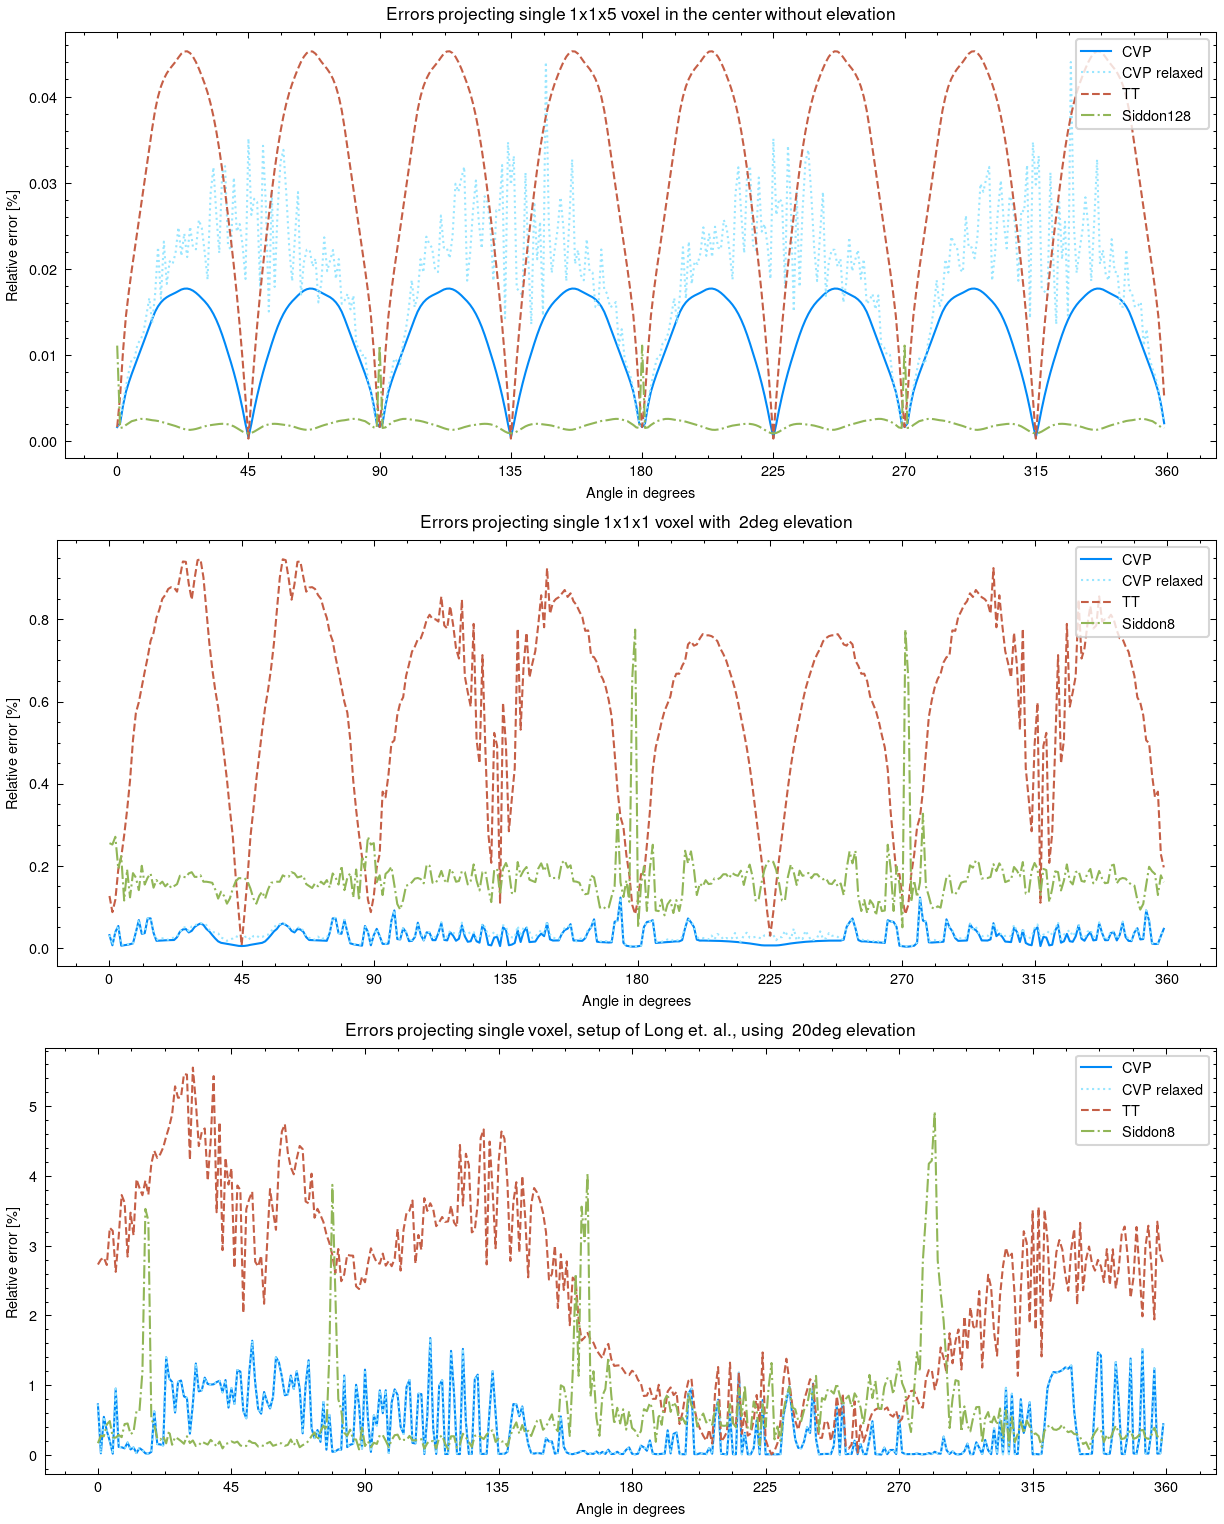
\includegraphics[width=\textwidth]{projectorComparison.png}
    \caption{Comparison of projection errors of different projectors at different settings. In the top image, the voxel is placed in the center of rotation is studied. In the middle image, the voxel is outside rotation center shifted so that the elevation and cone beam angles are around \SI{2}{\degree}. The bottom image shows a setup with  a voxel projected with a large cone beam angles and elevations.}
    \label{fig:projectorerror}
\end{figure*}

% \subsection{Transparency and reproducibility of the results}

% We believe in the concept of open science. Therefore, not only the software developed by the first author is published under an open source license, we are also publishing all the procedures, scripts, input data and log files, including implementation details, that were used to produce the graphs and tables in the results section. This way, anyone can reproduce our steps on their hardware and compare the results, or use our logs and scripts to compare the results with the underlying data. The files and protocols are published on the website \url{https://kulvait.github.io/KCT_doc/categories/cvp-paper-2021.html}.

% This is also important for the users of the software, because in the future we can disclose how the run times of the projectors change with new versions of the software or with new hardware.



%For studying the properties of cutting voxel projector under various scanning settings and discretizations of the volume and  we have chosen two configurations based on the diagnostic trajectories of the Artis Q SIEMENS C-Arm CT system for the brain tomographic scanning, where the distance from the source to the isocenter is $\SI{749}{\milli \meter}$ and the distance from source to the detector is $\SI{1198}{\milli \meter}$. Detector matrix of the device consists of $2464 \times 1920$ detector cells of the dimensions $\SI{0.154}{\milli \meter} \times \SI{0.154}{\milli \meter}$. For the purposes of the tomographic reconstruction there is applied tiling of the pixels, the procedure where the signal is obtained from the merged pixels of the size either $2 \times 2$ or $4 \times 4$.

%Setup I. is derived from the brain scan and uses tiling $2 \times 2$ with merged pixel size of $\SI{0.308}{\milli \meter} \times \SI{0.308}{\milli \meter}$. The trajectory consists of $496$ source and the detector geometrical configurations from which are obtained projection data of the size $1232 \times 960$ pixels. Setup II. is derived from the brain perfusion scan and uses tiling $4 \times 4$ with merged pixel size of $\SI{0.616}{\milli \meter} \times \SI{0.616}{\milli \meter}$. The trajectory consists of $248$ source and the detector geometrical configurations from which are obtained projection data of the size $616 \times 480$ pixels. 

%Siemens was using 0.46433800458908x0.46433800458908x0.46433800458908 voxels in the grid 512x512x325 = 238x238x151
%Siemens was using 0.46433800458908x0.46433800458908x0.46433800458908 voxels in the grid 512x512x394 = 238x238x182
%0.95545232421875x0.95545232421875x0.95545232421875 voxels in the grid 256x256x184 =245x245x175
%(0018, 1100) Reconstruction Diameter = 512 The diameter defines a circular region that is entirely contained within the encoded Pixel Data (7FE0,0010), unless the encoded image has been cropped after reconstruction. 
%As a testing volumes, we have chosen two volumes of the Shepp-Logan 3D like phantom and one volume of the realistic brain phantom, see \cite{Aichert2013}. Shepp-Logan 3D phantom volumes were generated with the voxels that are longer in z-axis direction than xy-axis direction to test this common setup, while the realistic head phantom volume has uniform voxel sizes in every direction so that the volume is in the form proposed by the authors of \cite{Aichert2013}.

%First we have generated Shepp-Logan 3D like phantom of the dimensions $1024 \times 1024 \times 1024$ with the voxel size $\SI{0.215}{\milli\meter} \times \SI{0.215}{\milli \meter} \times \SI{0.215}{\milli \meter}$ that represents the volume of the size $\SI{220.16}{\milli\meter} \times \SI{220.16}{\milli \meter} \times \SI{220.16}{\milli \meter}$. We interpolated this volume to the two different grids of the sizes $256 \times 256 \times 64$ and $512 \times 512 \times 128$ which correspond to the voxel sizes $\SI{0.86}{\milli \meter} \times \SI{0.86}{\milli \meter} \times \SI{3.44}{\milli \meter}$ and $\SI{0.43}{\milli \meter} \times \SI{0.43}{\milli \meter} \times \SI{1.72}{\milli \meter}$ respectively.

%For the realistic brain phantom we have generated the volume by the procedure described in \cite{Aichert2013}. Size of the volume without slices containing zeros is $256\times256\times212$. For voxels of the dimensions $\SI{0.9}{\milli \meter} \times \SI{0.9}{\milli \meter} \times \SI{0.9}{\milli \meter}$ the grid fits into the volume of $\SI{230.4}{\milli\meter} \times \SI{230.4}{\milli \meter} \times \SI{190.8}{\milli \meter}$.


%For each discretized volume and setup we first compute its projections using given projector. Then we run constant number of $40$ iterations of CGLS algorithm for the tomographic reconstruction. Then we study the norm of residuum, norm of error based on the original data and computational time of reference implementation.


%For each volume discretization we first resized original volume and compute projections using given projector backprojector pair.

%We decided to test cutting voxel projector by comparing the reconstructions created using d

\section{Discussion}

The cutting voxel projector (CVP) algorithm, based on the principles in \cref{sec:cuts}, was first implemented in 2019. Since its inception, it has been employed in hundreds of reconstruction problems, particularly in improving algorithms for processing CBCT perfusion data. Notably, it has contributed to prior works such as \cite{Kulvait2021, Haseljic2021, Kulvait2022}. Throughout its applications, the projector has consistently demonstrated high accuracy, comparable to or exceeding the established TT footprint projector, especially for complex cone-beam geometries. 

More recently, the algorithm has been adapted for parallel-ray geometry, where the absence of elevation correction requirements makes it an almost exact projector, e.g. for synchrotron $\mu$-CT setups, see also \cite{Moosmann2014}. This extension underscores its versatility and accuracy across a broader range of tomographic applications. The GitHub repository with the implementation is often cloned and has 19 stars as of November 2024.

\subsection{Elevation correction}
When comparing projector profiles across elevation angles, as seen in \cref{fig:projectorerror}, the CVP exhibited consistently low errors but occasionally showed localized spikes above the TT projector. Closer examination revealed that these errors occurred at the top or bottom edges of voxel projections and were associated with how the center of mass of the voxel's slice aligned with pixel boundaries in the $\chi_2$ direction.

To address this, we introduced an elevation correction. This modification extends the projected line (defined by the center of mass and $x_3$ limits) into a rectangle, allowing a portion of the projection to be assigned to the appropriate pixel. While this increases computational complexity, it also improves accuracy without a substantial impact on runtime, particularly for the relaxed version of the projector.

For most use cases, especially those with small cone angles, the CVP without elevation correction remains a very good choice, offering high accuracy with fast performance. However, for applications with large cone angles or precise scenarios requiring maximum accuracy, the elevation correction provides clear benefits, as shown in \cref{fig:projectorerror}.

\subsection{Speed and GPU optimization}
Tables \ref{speed:long} and \ref{speed:pfeiffertest} highlight the impressive runtime performance of the CVP, particularly its relaxed variant. Achieving these results required GPU-specific optimizations, including computing cuts in the $x_1x_2$ plane separately for each voxel. This strategy aligns well with GPU architectures, enabling effective parallelization by assigning one thread per voxel. Furthermore, optimized memory conflict handling in the local GPU memory was implemented to minimize memory access contention and maximize computational throughput.

Despite these optimizations, the projector remains slower than the backprojector. For speed sensitive use cases, it may be advisable to relax the accuracy requirements of the forward projector and use a fast, low-accuracy ray-tracing method. The backprojector, however, cannot be similarly simplified, as doing so would amplify operator inaccuracies, particularly in iterative reconstruction methods. Frameworks like ASTRA, see \cite{ASTRA2016}, often adopt this strategy, combining a forward raytracer and a backward footprint projector for speed efficiency, even at the cost of sacrificing the self-adjointness of the tomographic operator.

\subsection{Possible Improvements}
While the CVP algorithm has been extensively optimized, these improvements are possible in case of footprint projectors as well. For example, applying the same parallelization techniques used in the CVP to footprint projectors, such as the TT or TR projectors, could significantly accelerate their performance. Current implementations, such as the approach described by Long et al. \cite{Long2010}, are primarily CPU-optimized and do not fully exploit GPU capabilities. By restructuring the calculations to parallelize over voxels rather than rows and columns, as demonstrated in our CVP implementation, significant speedups could likely be achieved for these projectors as well.

%Additionally, for applications requiring extremely precise reconstructions and involving large cone angles, the role of elevation correction becomes increasingly important. Future work will investigate the performance of the elevation-corrected CVP in such scenarios to determine its potential benefits in these high-accuracy use cases.

In future work, we plan to explore the application of the CVP to non-circular trajectories. While the current implementation in \cref{sec:implementation_full} assumes alignment between the voxel $x_3$ axis and the detector $\chi_1$ axis, the derivation in \cref{sec:formulation} is independent of this. By leveraging algorithms for computing general cube and square pyramid intersections, it would be possible to construct projectors for arbitrary scanning trajectories, distinguishing the CVP from footprint projectors that inherently rely on this geometric alignment by design.

\subsection{Conclusion}
This work introduces and evaluates a cutting voxel projector that balances speed and accuracy, outperforming existing projectors like TT and Siddon's algorithm for CBCT geometries. The elevation-corrected CVP is presented as the most accurate known projector, except for extremely computationally expensive ray-tracing approaches. Its GPU-optimized implementation and superior runtime performance make it a promising tool for advancing algebraic reconstruction techniques.

A key advantage of the proposed cutting voxel projector lies in its support for hierarchical reconstruction with nonuniform voxel grids. This flexibility opens the door to developing advanced computational techniques analogous to algebraic multigrid (AMG) methods used in solving partial differential equations. By enabling local voxel refinement, the projector provides the groundwork for adaptive tomographic reconstruction approaches that can focus computational resources on regions of interest while maintaining coarser resolution elsewhere. In future work, we aim to leverage this capability to design hierarchical solvers for the tomographic reconstruction problem, incorporating multigrid-inspired strategies such as dynamic grid coarsening and refinement. These developments hold the promise of significantly improving the scalability and efficiency of algebraic reconstruction techniques, particularly for large-scale or high-resolution imaging tasks. The cutting voxel projector thus not only delivers improved accuracy and performance today but also establishes a foundation for transformative innovations in adaptive tomographic reconstruction techniques.

\section*{Acknowledgments}
V. Kulvait (VK) designed and implemented the cutting voxel projector for the CBCT operator during his postdoctoral position at OVGU. Later, while serving as a scientist at Hereon, he developed a simplified version for parallel beam geometry tailored for synchrotron $\mu$-CT applications. The OpenCL kernels are now included in the open-source package for tomographic reconstruction, KCT\_cbct. The implementations are publicly available as open-source software under the GNU GPL 3 license at \url{https://github.com/kulvait/KCT_cbct}.

\bibliographystyle{siamplain}
\bibliography{literature}
\end{document}
